\section{Preprocessing}
\label{sec:preprocessing}
This section discusses some preprocessing techniques before we actually carry out the stitching. The X-ray images might not be perfect for stitching; the noise present in the image cause inaccurate stitching, the high resolution images are slower or sometimes the intensity different between the images gives unpleasant stitched result. The X-ray images should be preprocessed before they are input for feature extraction. For image stitching problem, we generally focus on the following preprocessing steps:
\begin{description}
	\item [Noise Reduction] The noise in the image gives inaccurate result; so noise reduction is a crucial step in stitching. There are several smoothing operators (see section~\ref{sec:image-smoothing}) which can be implemented to suppress the noise in the image. The smoothing should not reduce the image information that we use for stitching. So, experimentally decide the effective image smoother and its parameters.
	
	\item [Intensity Leveling] To get the better stitching result, the images to be stitched should have similar intensity. The intensity differences in the images actually effects the key points identification process because the same image with different intensities result different key points. Similarly, we have to implement more effective blending operations because different intensity images generate a visible seam in the join of images. So, intensity leveling technique makes the image intensities similar to get better stitching result. 
	\item [Overlapping Area Prediction \& Selection] Sometimes, if we already know some information regarding alignment, we can use this information to simplify the image stitching task. For X-ray images, images are always either aligned vertically or horizontally. So, if images are aligned horizontally, we can predict that the second half of the first image and first half of the second image have high probability of overlapping. We select the second half of first image and first half of the second image for faster estimation of motion parameters. 
\begin{figure}%
\centering
\subfloat[]{%
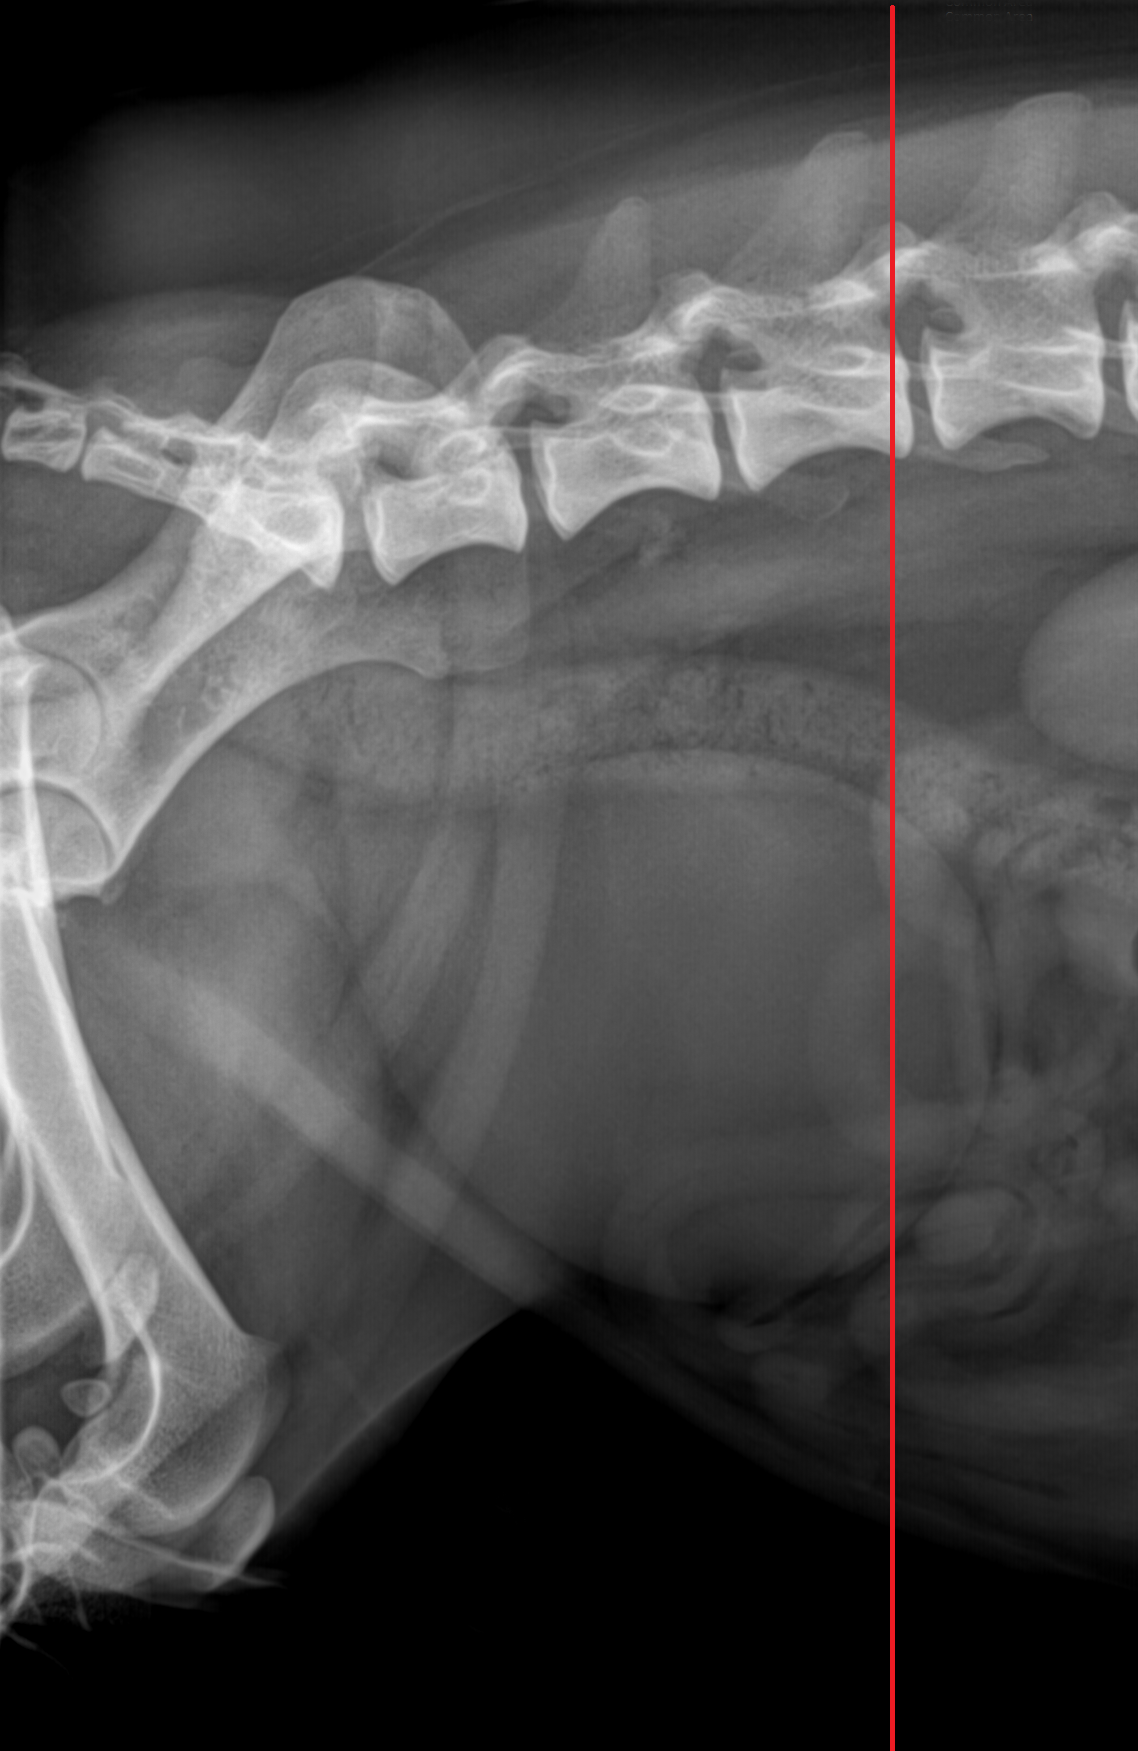
\includegraphics[scale=0.15]{2.mainmatter/2.Methodology/figures/left}
\label{fig:left}%
}
\qquad
\subfloat[]{%
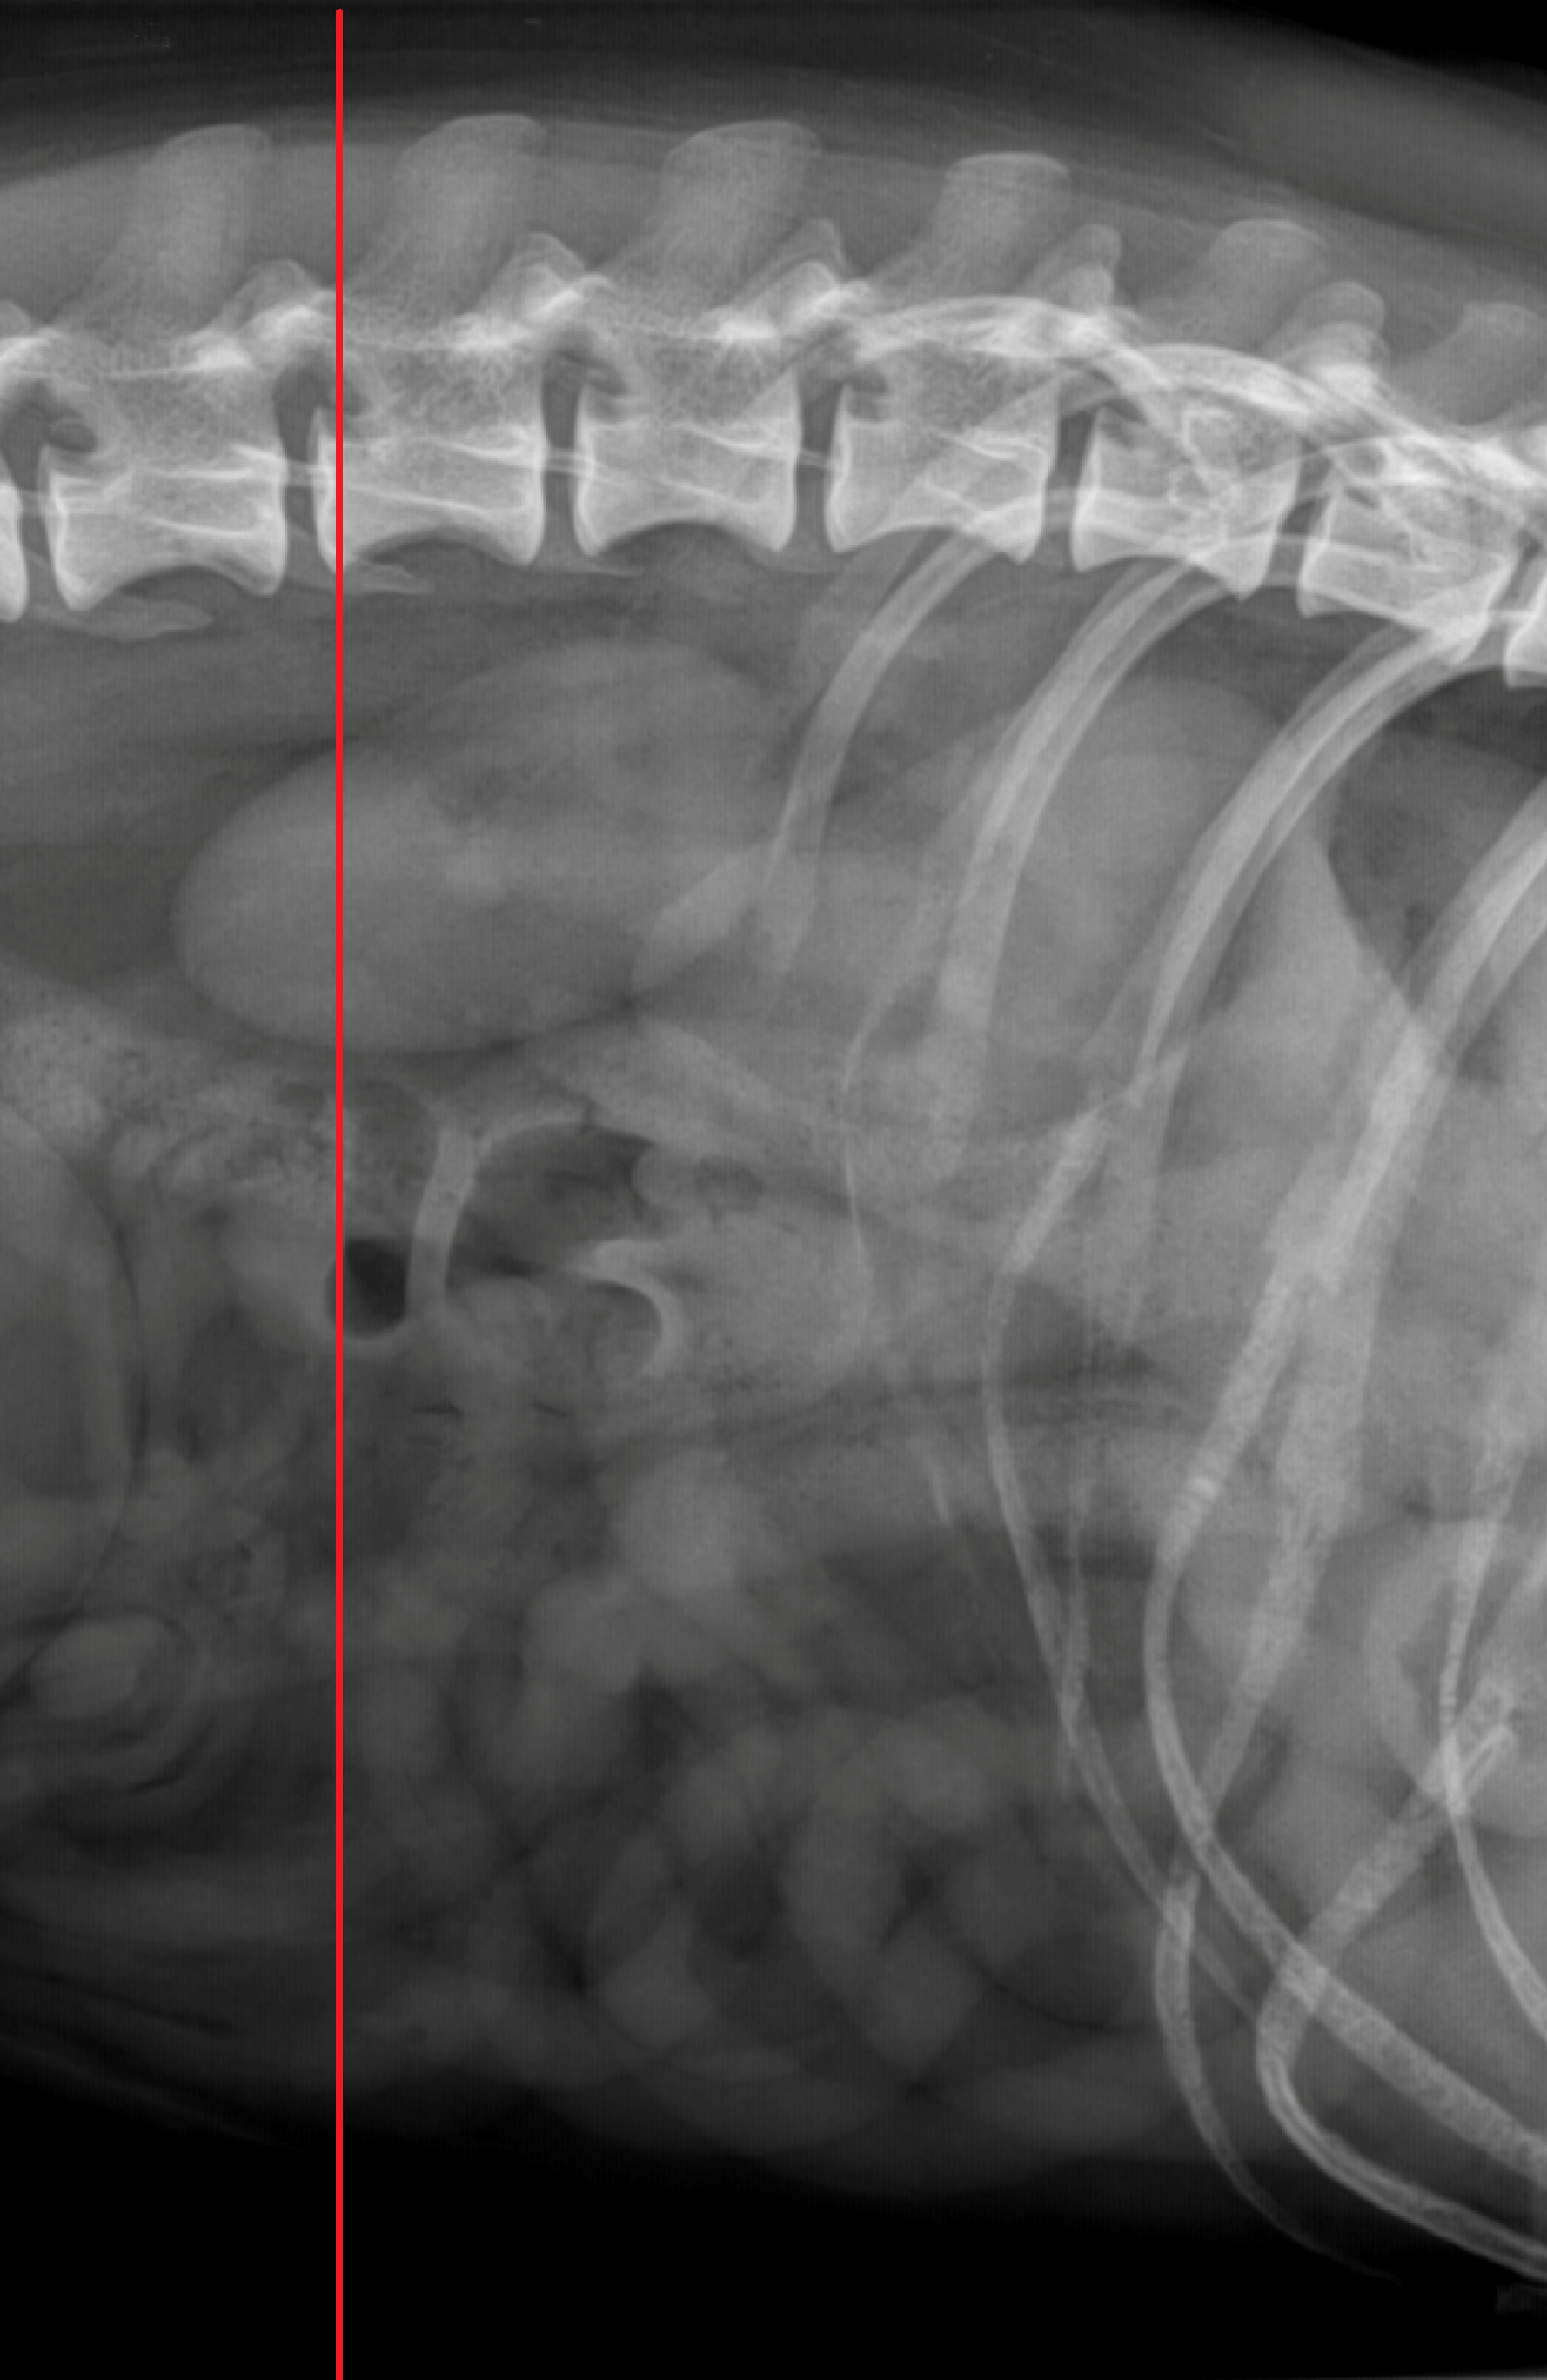
\includegraphics[scale=0.15]{2.mainmatter/2.Methodology/figures/right}%
\label{fig:right}%
}%
\caption[Overlapping Area Prediction]{The second half of figure~\subref{fig:left} and the first half of figure~\subref{fig:right} chosen for faster estimation of motion parameters. The vertical line separates the overlapped region.}%
\label{fig:overlap-estimation}%
\end{figure}	
\end{description}

%Intensity levelling
%Noise Reduction
%Cropping Unnecessary Parts
